\section{Real-Time Deployment}
\label{sec:deployment}
% =============================================================================

We validate the committed-action framework in a two-GPU real-time setup
across real-time Tetris, Pac-Man, and Snake. One GPU runs the
environment and executes committed actions continuously; the second runs
MCTS. At each meta-decision the current game state is transferred to
the planning GPU, which searches while the environment GPU keeps the
game moving. When planning finishes, after $K \times 32$ simulations,
the resulting action is applied at the next environment step
(Figure~\ref{fig:deployment_timeline}).

Figure~\ref{fig:deployment} summarizes 45 measured deployments:
3 environments $\times$ 3 GPU classes $\times$ 5 frame rates (8--12\,FPS).
The asynchronous execution pattern is unchanged from training: a $K{=}4$
meta-step at 9\,FPS spans four 111\,ms frames, while reflex actions keep the
environment moving and MCTS finishes asynchronously on the second GPU.

The main result is that simulation-trained policies transfer cleanly to
asynchronous hardware deployment over a broad operating range. Latency
stays within budget on H100 in all three environments, and remains
reliable on A100 except near the tightest deadlines. Return transfer is
also strong: at 9\,FPS, deployed returns remain close to their
simulation counterparts, and the learned budget distribution carries
over as well. In Tetris on H100, the deployed policy preserves the same
strongly bimodal ``react or plan deeply'' strategy seen in simulation.
Appendix~\ref{app:deployment_details} gives the full breakdown by
environment, FPS, and GPU.

This result validates the committed-action training protocol. Because
training already simulates planning delay by executing committed
actions, the learned policy transfers to asynchronous deployment
without modification. A fixed 1-step RTMDP formulation
~\citep{ramstedt2019rtrl} is not expressive enough for variable-budget
MCTS spanning $K \in \{1,\ldots,4\}$ frames; a naive extension would
need to carry a variable number of stale actions in the state. Appendix
~\ref{app:rtrl_smdp} discusses this point in more detail.

\begin{figure}[h]
  \centering
  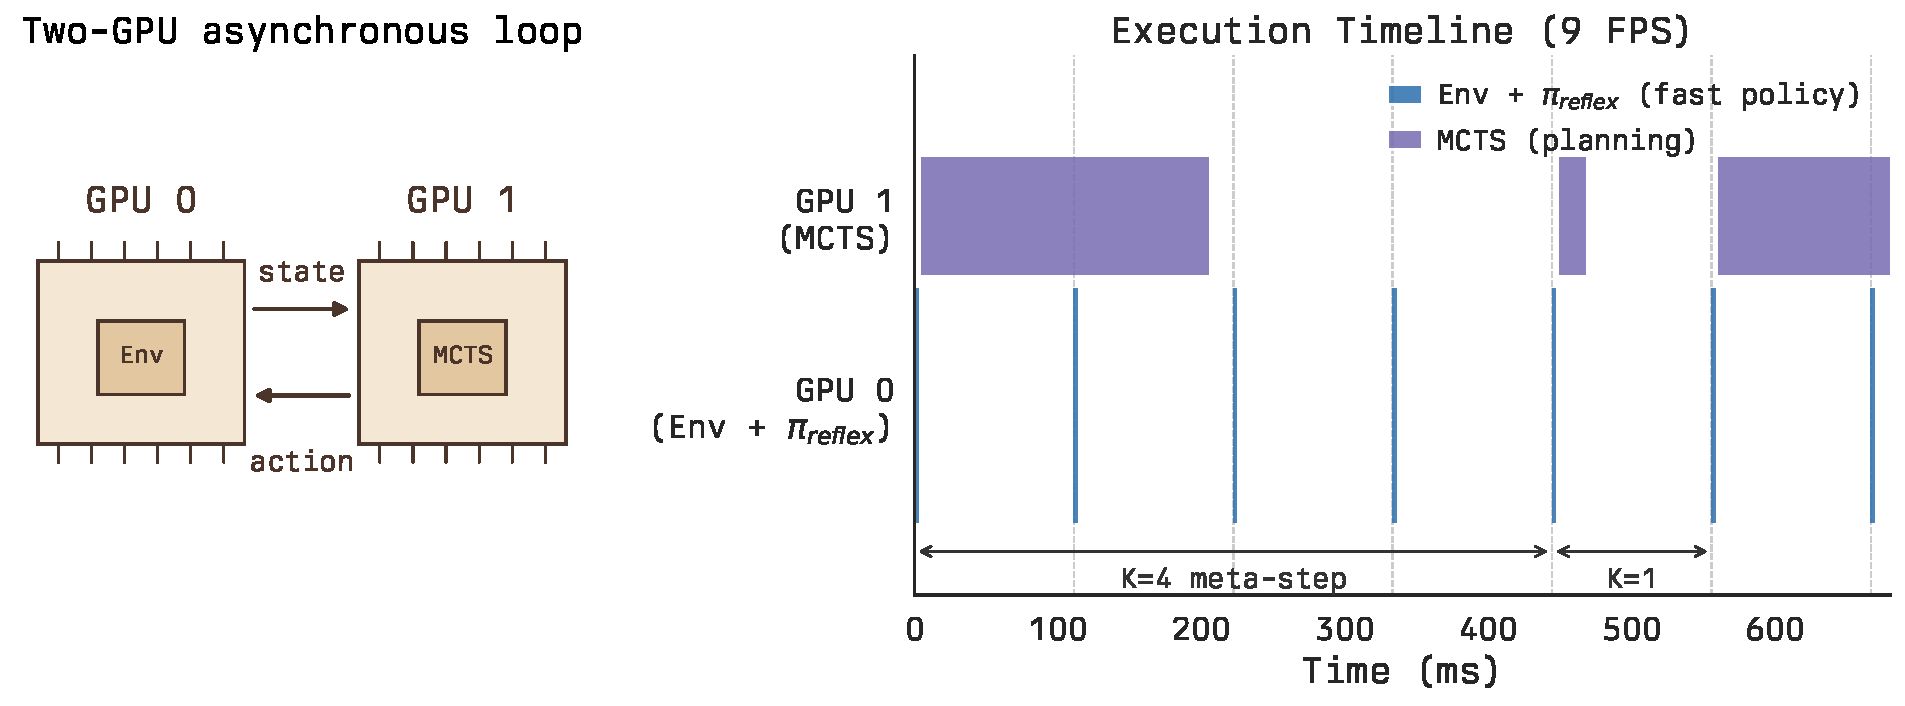
\includegraphics[width=\linewidth]{figures/deployment_timeline.pdf}
  \caption{\textbf{Two-GPU real-time deployment pipeline.}
    GPU~0 runs the environment continuously via committed (reflex) actions;
    GPU~1 runs MCTS in parallel, so a larger $K$ buys more planning time without
    pausing the game.
    \emph{Left:} schematic of the two-GPU loop.
    \emph{Right:} execution trace at 9\,FPS---a $K{=}4$ meta-step spans four 111\,ms
    frames, followed by a $K{=}1$ recovery step.}
  \label{fig:deployment_timeline}
\end{figure}

\begin{figure}[h]
  \centering
  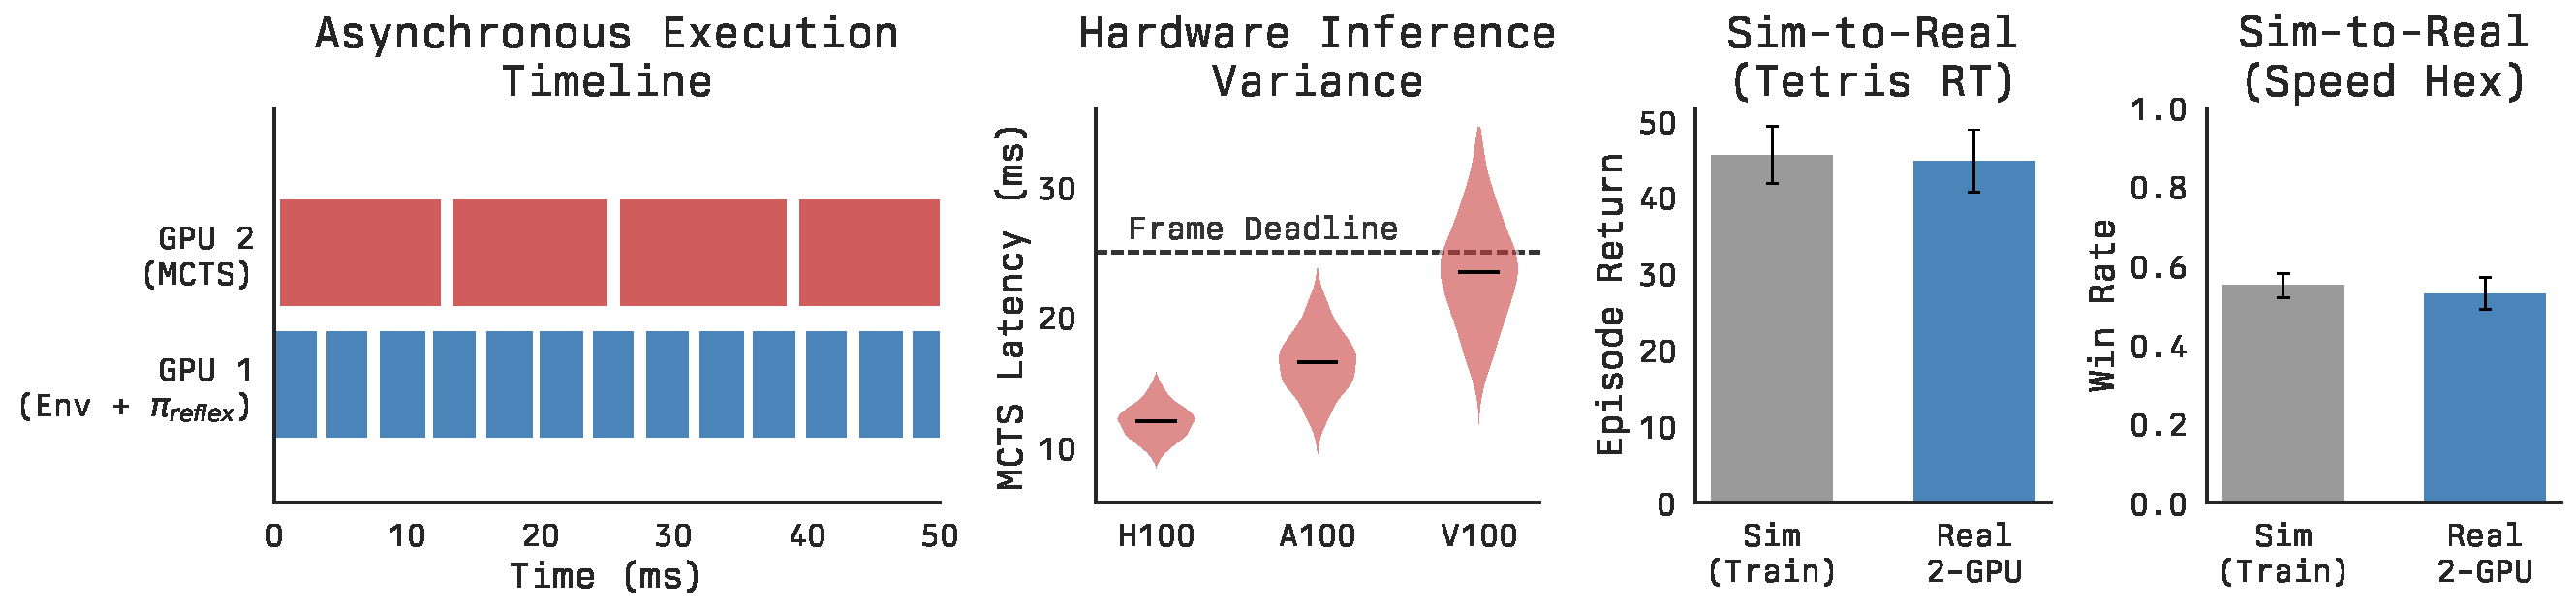
\includegraphics[width=\linewidth]{figures/deployment.pdf}
  \caption{\textbf{Simulation-trained policies transfer cleanly to hardware deployment.}
    \emph{Left:} MCTS latency variance tightens with GPU class---H100 is most
    consistent, A100 intermediate, A40 widest.
    \emph{Centre:} H100 and A100 miss deadlines rarely; A40 breaks down only at
    the tightest frame rates.
    \emph{Right:} Deployed returns at 9\,FPS match simulation closely across all
    environments and GPU classes.
    See Appendix~\ref{app:deployment_details} for the full breakdown.}
  \label{fig:deployment}
\end{figure}

% =============================================================================
